% Overleaf-ready. Compile with pdflatex (Overleaf default) or tectonic. No extra fonts required.
\documentclass[11pt,a4paper]{article}

\usepackage[margin=2.5cm]{geometry}
\usepackage[T1]{fontenc}
\usepackage[utf8]{inputenc}
\usepackage{lmodern}
\usepackage{microtype}
\usepackage{amsmath}
\usepackage{booktabs}
\usepackage{graphicx}
\usepackage{tabularx}
\usepackage{array}
\usepackage{caption}
\usepackage{float}
\usepackage{enumitem}
\usepackage{xcolor}
\usepackage{csquotes}
\usepackage[hyphens]{url}
\usepackage{hyperref}

\hypersetup{
  colorlinks=true,
  linkcolor=black,
  citecolor=black,
  urlcolor=blue,
  pdftitle={Airtel Kenya customer-message classifier},
  pdfauthor={Christopher Kioko}
}

\graphicspath{{figures/}}


\setlength{\parindent}{0pt}
\setlength{\parskip}{0.55em}
\emergencystretch=3em
\setlist[itemize]{topsep=0.3em, itemsep=0.2em, leftmargin=1.4em}
\setlist[enumerate]{topsep=0.3em, itemsep=0.35em, leftmargin=1.4em}
\captionsetup{font=small, labelfont=bf, skip=6pt}

\title{Airtel Kenya customer-message classifier}
\author{Christopher Kioko}
\date{November 2026}

\begin{document}

\begin{titlepage}
  \centering
  \vspace*{2.2cm}
  {\Large Strathmore University\par}
  \vspace{0.9cm}
  {\large DSA 8401 Applied Machine Learning\par}
  \vspace{2.2cm}
  {\Huge\bfseries Airtel Kenya customer-message classifier\par}
  \vspace{0.8cm}
  {\large Capstone report\par}
  \vspace{2.4cm}
  {\Large Christopher Kioko\par}
  \vspace{0.6cm}
  {\large November 2026\par}
  \vfill
  {\large Clearance status: it is cleared for coursework.\par}
  \vspace{0.8cm}
\end{titlepage}

\section*{Clearance and scope}

DSA 8401 capstone. Christopher Kioko. Clearance status: it is cleared for coursework.

No customer message is quoted in this report. Counts and metrics are aggregates.

\section{Problem framing}

Airtel Kenya's customer-care queue receives short messages in English, Swahili, and Sheng. Each message needs three decisions at once: what the customer is asking about (10 issue classes), whether the tone is negative, and how quickly the message should move (low, medium, or emergency). The messages are raw exports, not a cleaned benchmark. Missing text, receipts, duplicates, and label leakage are part of the problem.

The live demo schema is the three-head JSON in \href{https://github.com/ChristopherKiokoStrathmore/MULTI-HEAD-}{MULTI-HEAD-}, file \texttt{lib/\allowbreak{}types.ts}. This repository trains and serves that schema.

\section{Data}

The workbook is one sheet, 526,369 rows by 29 columns, posted from November 2025 through April 2026. Channels are Airtel Kenya page variants and the Twitter handles. \texttt{prepare\_\allowbreak{}data} keeps the original channel and type beside a normalised form, masks PII as \texttt{[PHONE]}, \texttt{[URL]}, \texttt{[USER]}, and \texttt{[ID]}, and drops rows that fail the inclusion rules.

Real workbook audit:

\begin{table}[H]
\centering
\caption{Workbook inclusion audit (row counts).}
\begin{tabular}{lr}
\toprule
 & rows \\
\midrule
in & 526,369 \\
kept & 379,575 \\
empty & 47,004 \\
non-linguistic & 98,317 \\
auto receipts & 1,473 \\
\bottomrule
\end{tabular}
\end{table}

Label files are already masked. Original names and the loader names are in \texttt{docs/\allowbreak{}label\_\allowbreak{}rubric.md} and \texttt{FILE\_\allowbreak{}MAP}.

\begin{table}[H]
\centering
\caption{Label sources and real splits (train / validation / test).}
\small
\begin{tabularx}{\textwidth}{l>{\raggedright\arraybackslash}Xl}
\toprule
Head & Source & Real split (train / val / test) \\
\midrule
Issue & \texttt{issue\_\allowbreak{}retagged\_\allowbreak{}clean\_\allowbreak{}1500.csv}, 10 classes, retagged by Chris & 1,028 / 226 / 224 \\
Sentiment & hand labels in \texttt{sentiment\_\allowbreak{}judgment\_\allowbreak{}1500.csv}; test is \texttt{sentiment\_\allowbreak{}test\_\allowbreak{}to\_\allowbreak{}annotate(in).csv} & 1,215 / 260 / 150 \\
Urgency & \texttt{urgency\_\allowbreak{}v3\_\allowbreak{}train (2).csv} and \texttt{urgency\_\allowbreak{}v3\_\allowbreak{}test (2).csv} & 794 / 60 / 120 \\
\bottomrule
\end{tabularx}
\end{table}

Urgency validation is 60 rows and every one of them is gold. The 120-row test is the fixed gold file. 688 urgency training rows are Groq silver (\texttt{source=distilled}) and are down-weighted. Gemini's \texttt{gemini\_\allowbreak{}relabeled.csv} is not a training source.

Platform sentiment versus hand sentiment, recomputed: agreement 0.711 and kappa 0.427 on 1,499 unique normalised texts. Row-aligned on all 1,500 rows the same agreement is 0.711 and kappa is 0.428. The platform file is the agreement table only.

Exact overlaps, recomputed: 9 urgency-test messages also sit in the issue/sentiment 1,500, 23 sit in the Gemini file, and 0 sit in the urgency training file. Gold, including near-duplicates, is removed from every training and validation pool. Splits are grouped on \texttt{dup\_\allowbreak{}group\_\allowbreak{}id}, seed 42.

\section{Pipeline}

\texttt{prepare\_\allowbreak{}data.py} reads the workbook once, checks the required columns, writes parquet under \texttt{data/\allowbreak{}private/\allowbreak{}}, and writes an aggregate audit with no message text. Inclusion drops empty text, text with no letters, and auto receipts. Exact duplicates and near-duplicates share \texttt{dup\_\allowbreak{}group\_\allowbreak{}id} (character 3-gram MinHash, Dice at least 0.80).

\texttt{splits.py} writes a JSON manifest per head: row ids, the duplicate group, and the SHA-256 of each source file. \texttt{tests/\allowbreak{}test\_\allowbreak{}no\_\allowbreak{}leakage.py} fails if any exact or near-duplicate is in both test and train/validation.

Real data stays in git-ignored \texttt{data/\allowbreak{}private/\allowbreak{}}. The repository ships a seed-42 synthetic sample. \texttt{make smoke} runs the pipeline, the baselines, a one-step tiny encoder, and evaluation on that sample. Those numbers are a harness check.

\begin{figure}[H]
\centering
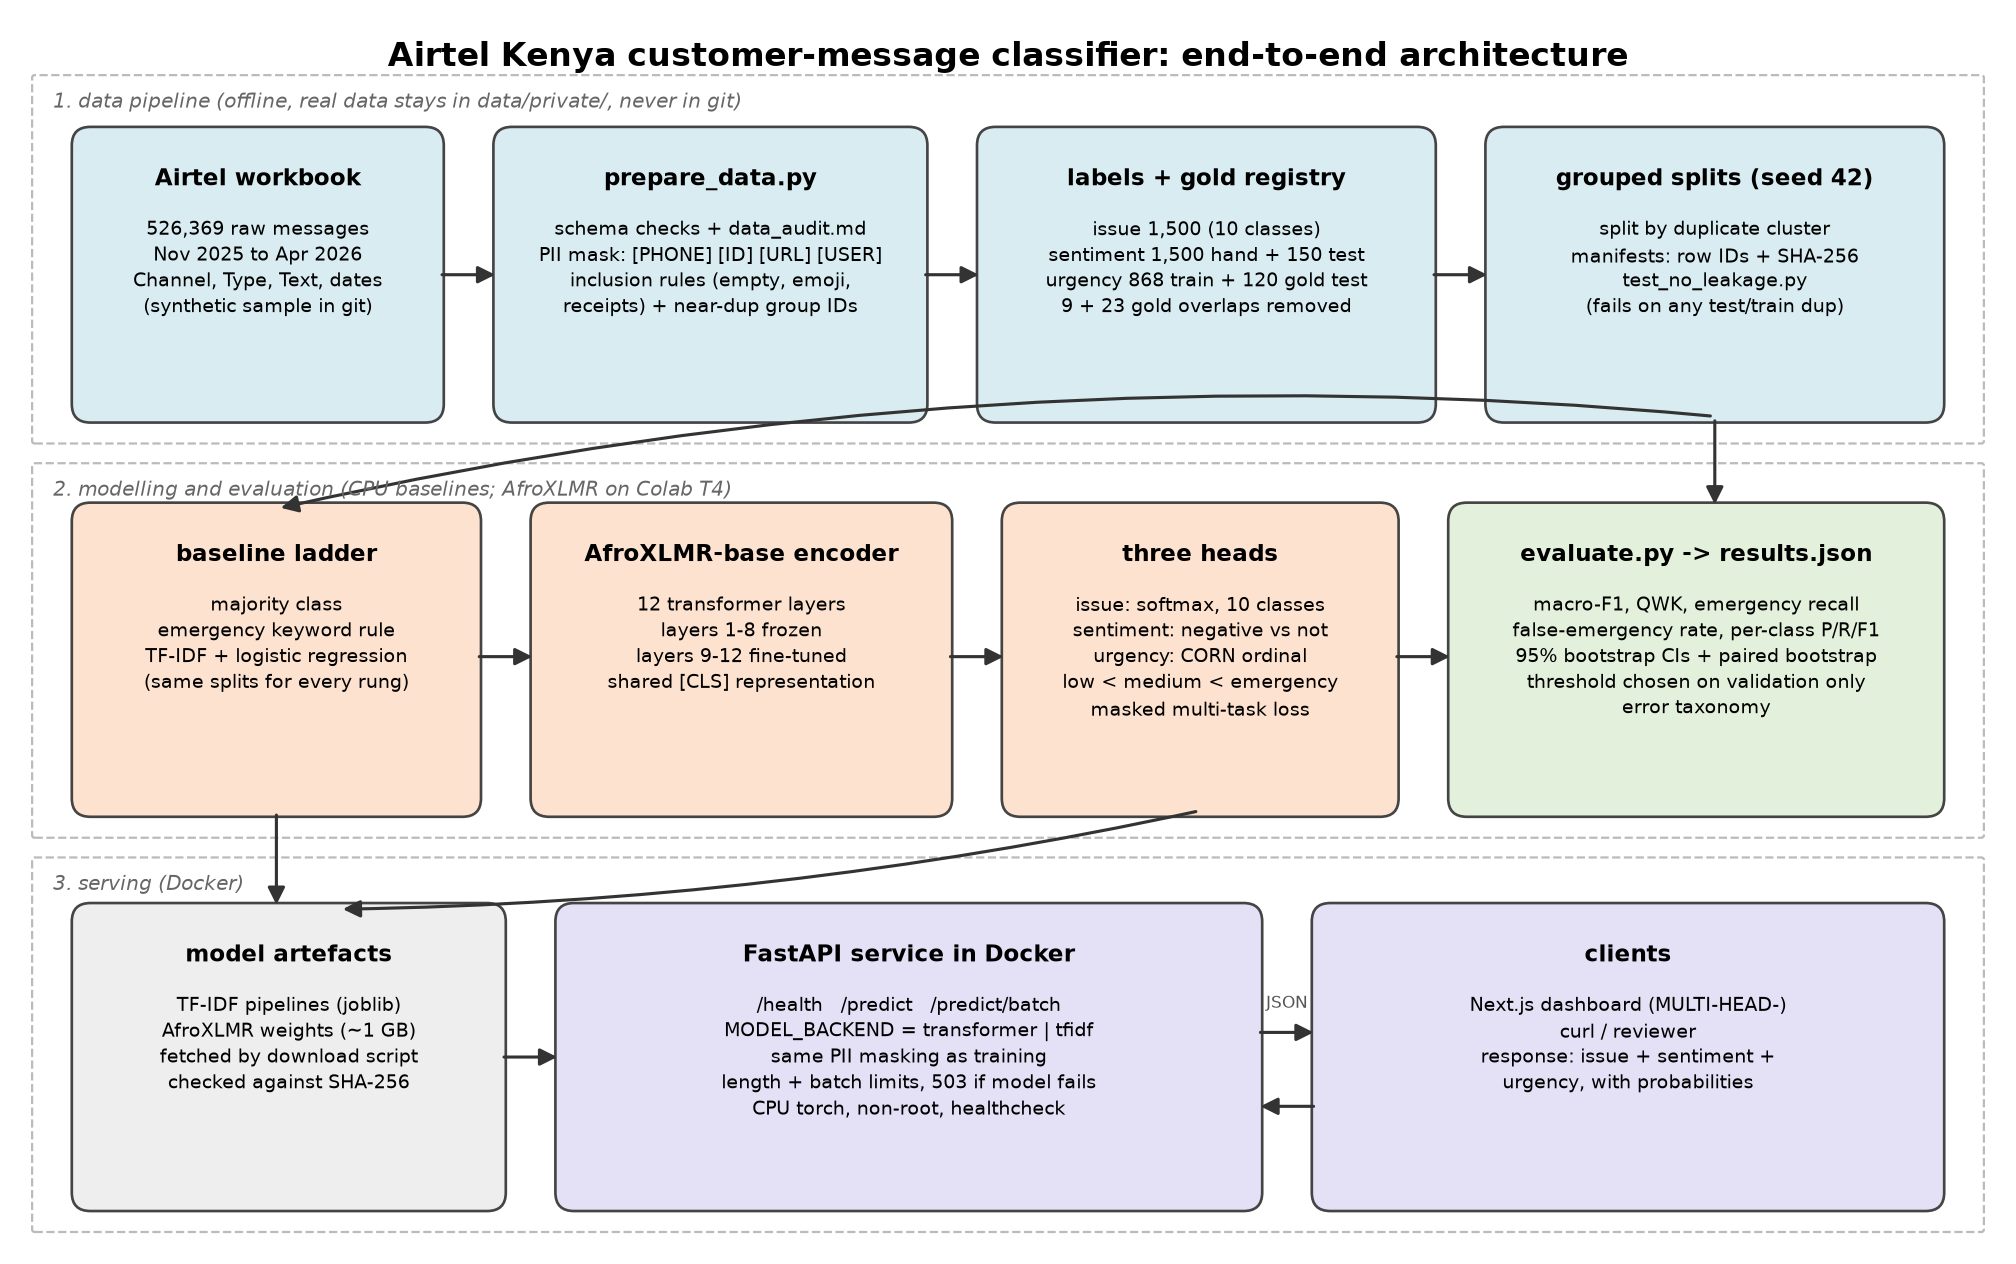
\includegraphics[width=\textwidth]{architecture.png}
\caption{Training pipeline: data, models, evaluation, and the Docker API (\texttt{docs/\allowbreak{}architecture.png}).}
\label{fig:architecture}
\end{figure}

\begin{figure}[H]
\centering
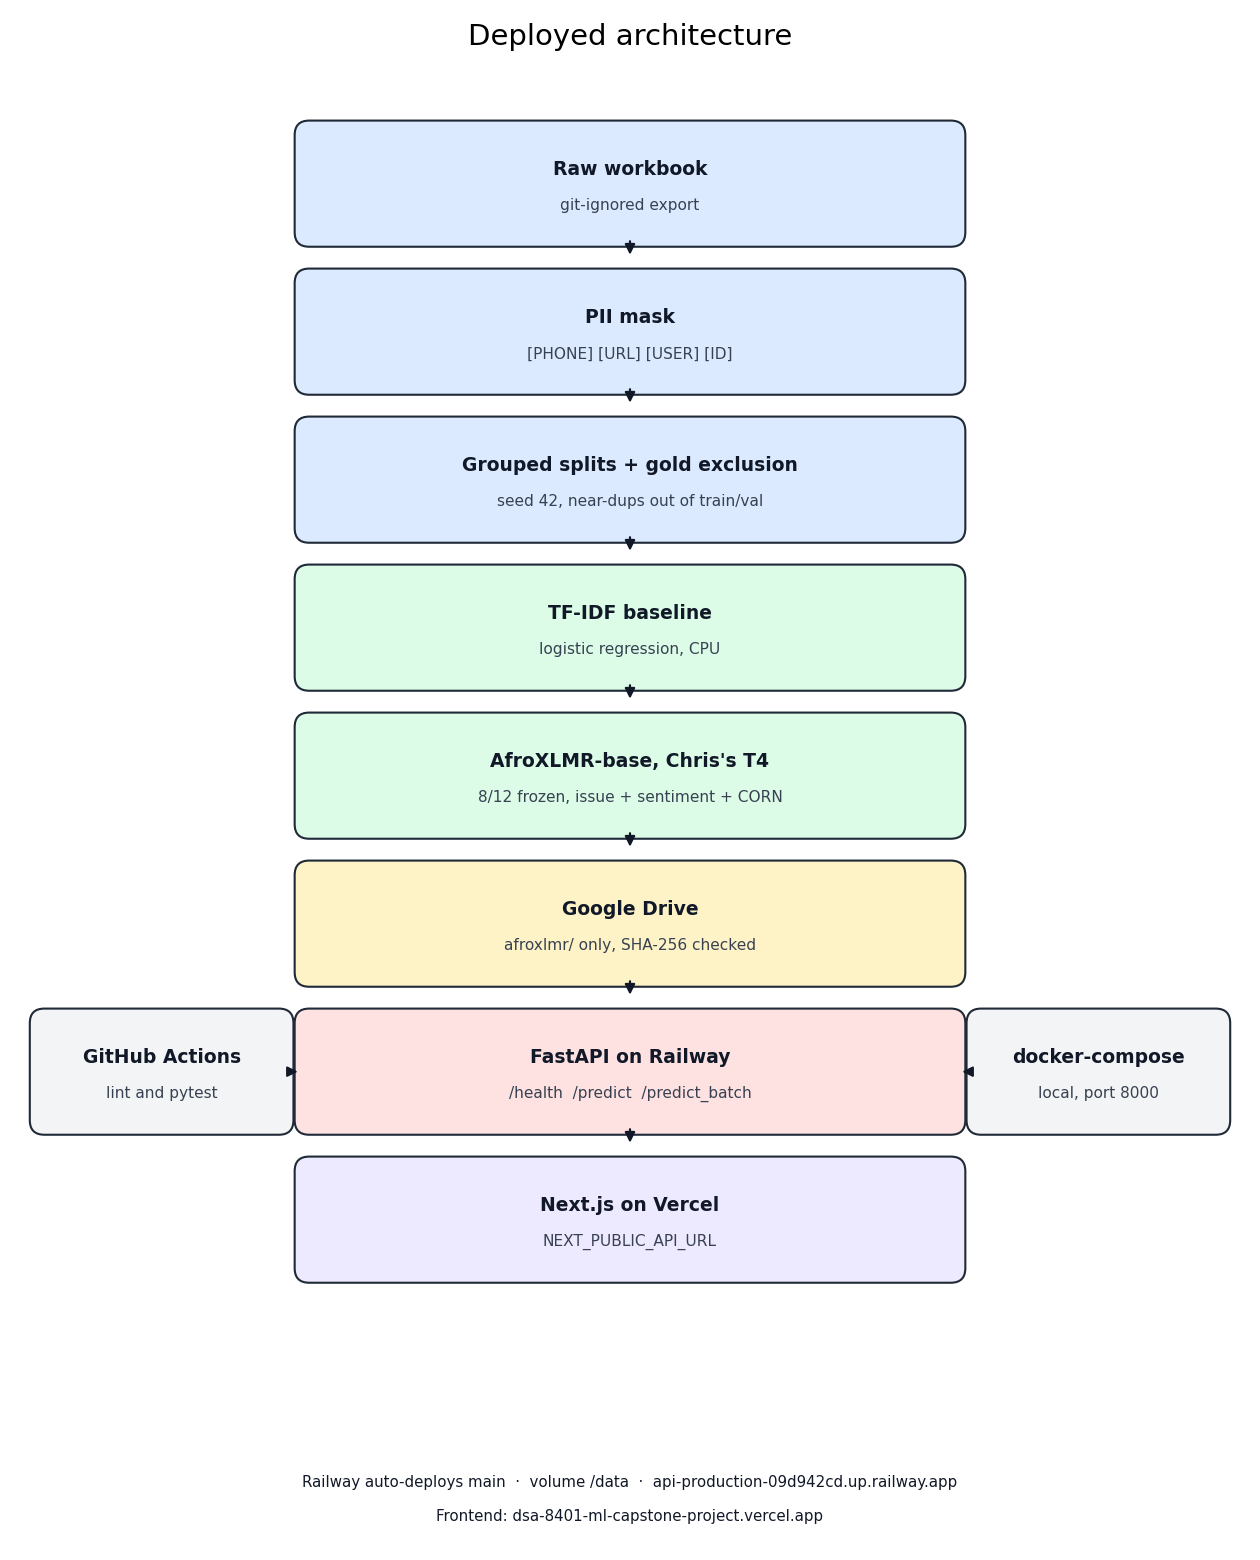
\includegraphics[width=\textwidth]{architecture-deployed.png}
\caption{Deployed path. Raw text is masked, split, and stripped of gold overlap. TF-IDF stays the CPU baseline. AfroXLMR-base (bottom 8 of 12 frozen, three heads, CORN urgency) was trained on one Colab T4. Weights sit on Google Drive and are SHA-256 checked into the Railway volume at \texttt{/data}. FastAPI (\texttt{/health}, \texttt{/predict}, \texttt{/predict\_batch}) is the Docker service at \url{https://api-production-09d942cd.up.railway.app}, auto-deployed from \texttt{main}. The Next.js app at \url{https://dsa-8401-ml-capstone-project.vercel.app/} calls it through \texttt{NEXT\_PUBLIC\_API\_URL}. GitHub Actions runs lint and pytest. \texttt{docker-compose} is the local path on port 8000.}
\label{fig:deployed}
\end{figure}

\section{Models}

Every rung uses the same splits. Nothing is chosen on the test set.

\begin{enumerate}
  \item Majority class, fit on train.
  \item Keyword heuristic, with emergency, medium, and issue cues. Unmatched text falls back to the training majority.
  \item TF-IDF, word bigrams and character 3--5 grams, then logistic regression with balanced class weights. $C$ is chosen on validation only, then the pipeline is refit on train.
  \item AfroXLMR-base, one seed (42). Embeddings and the bottom 8 of 12 layers are frozen. The top 4 layers and three heads train: issue softmax, sentiment softmax, urgency CORN. Masked loss, class weights, and urgency row weights. Early stopping uses validation macro-F1 and quadratic weighted kappa. The Colab T4 run used all 6 planned epochs (1,140 steps, about 25 minutes) and did not stop early. Epoch 6 validation: issue macro-F1 0.5819, sentiment macro-F1 0.8935, urgency QWK 0.5817 (\texttt{reports/\allowbreak{}afroxlmr\_\allowbreak{}run/\allowbreak{}curves.json}). The checkpoint is \texttt{model.pt}, 1,112,288,438 bytes. SHA-256: \texttt{778246a3\allowbreak{}1841ac55\allowbreak{}4fbf574c\allowbreak{}fc42cc95\allowbreak{}79981b67\allowbreak{}fb85a8eb\allowbreak{}1814dbb6\allowbreak{}89ea9eb6}.
\end{enumerate}

Base rather than large is a size decision. The proposal froze 8 of 24 layers. Freezing 8 of 12 keeps that one-third trainable and fits one Colab T4. The deviation is recorded in \texttt{docs/\allowbreak{}technique\_\allowbreak{}justification.md}.

The emergency flag is a threshold on $P(\text{emergency})$. It is chosen on the urgency validation split to maximise recall subject to a false-emergency rate of at most 0.20, then applied once to test.

\section{Evaluation}

\texttt{evaluate.py} scores whichever artefacts exist. If \texttt{artifacts/\allowbreak{}afroxlmr} is missing, that model is \texttt{not evaluated} in \texttt{results.json} and the baselines are still scored. Metrics, on the test split only: macro-F1, per-class precision, recall, and F1 with support, confusion matrices, urgency quadratic weighted kappa, emergency recall, and false-emergency rate. Intervals are 95\% percentile bootstrap, 1,000 resamples, seed 42. Paired intervals compare each scored model with TF-IDF on the same resamples. Mistakes go to \texttt{data/\allowbreak{}private/\allowbreak{}errors.csv} with a category hint. Thirty of them are marked for the error taxonomy. The report does not copy message text out of that file.

\section{Results}

The tables are the real test-split evaluation (\texttt{reports/\allowbreak{}results.json}, \texttt{kind: data}). They are not the smoke harness. AfroXLMR figures are the Colab T4 checkpoint, seed 42. Rounded to three decimals the same way \texttt{evaluate.py} writes \texttt{results.md}.

Validation curves (\texttt{reports/\allowbreak{}afroxlmr\_\allowbreak{}run/\allowbreak{}curves.json}):

\begin{figure}[H]
\centering
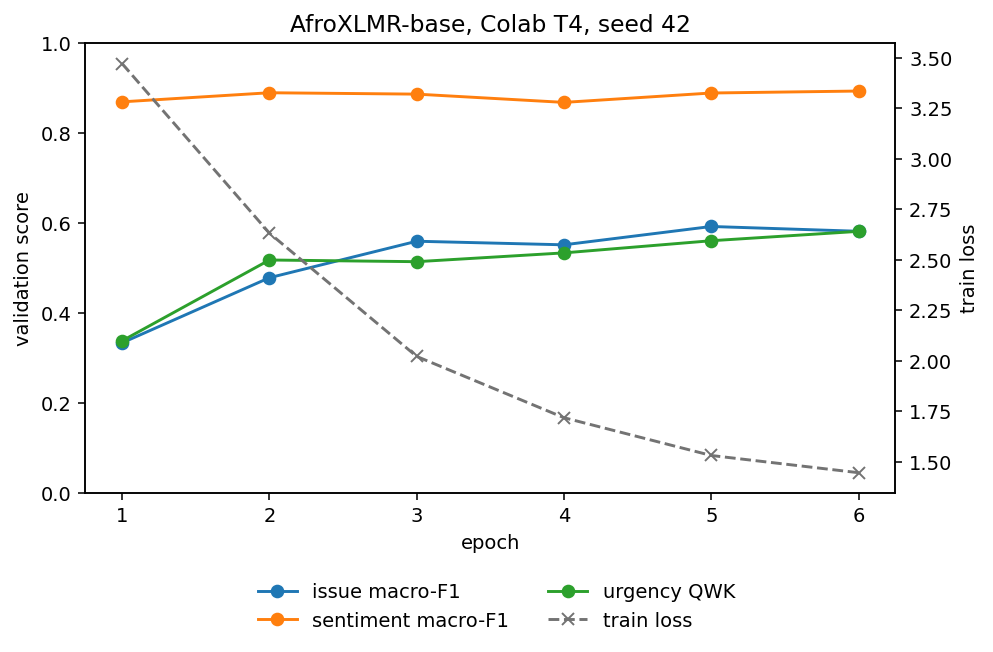
\includegraphics[width=0.92\textwidth]{learning_curves.png}
\caption{AfroXLMR validation curves on the Colab T4 run.}
\label{fig:curves}
\end{figure}

\begin{sloppypar}Emergency threshold on validation (real data). AfroXLMR's threshold is 0.50 (\texttt{reports/\allowbreak{}afroxlmr\_\allowbreak{}run/\allowbreak{}threshold.json}): validation emergency recall 0.810, false-emergency rate 0.179, under the 0.20 cap.\end{sloppypar}

\begin{table}[H]
\centering
\caption{Emergency threshold chosen on validation. The cap is a false-emergency rate of at most 0.20.}
\begin{tabular}{lcccc}
\toprule
model & threshold & val recall & val false-emergency rate & met cap \\
\midrule
majority & 0.95 & 0.000 & 0.000 & yes \\
keyword  & 0.80 & 0.095 & 0.026 & yes \\
tfidf    & 0.45 & 0.714 & 0.154 & yes \\
afroxlmr & 0.50 & 0.810 & 0.179 & yes \\
\bottomrule
\end{tabular}
\end{table}

\subsection{Issue (\texorpdfstring{$n = 224$}{n = 224})}

\begin{sloppypar}Gold support: \texttt{Airtel\_\allowbreak{}Money\_\allowbreak{}Reversal} 4, \texttt{Airtel\_\allowbreak{}Money\_\allowbreak{}Transfer} 19, \texttt{App\_\allowbreak{}Rewards} 14, \texttt{Complaint\_\allowbreak{}General} 6, \texttt{Data\_\allowbreak{}Bundle\_\allowbreak{}Problems} 22, \texttt{Network\_\allowbreak{}Issues} 41, \texttt{Non\_\allowbreak{}Actionable} 57, \texttt{Product\_\allowbreak{}Enquiry} 20, \texttt{Router\_\allowbreak{}WiFi\_\allowbreak{}5G} 21, \texttt{SIM\_\allowbreak{}Line\_\allowbreak{}Services} 20.\end{sloppypar}

\begin{table}[H]
\centering
\caption{Issue-head test macro-F1 with 95\% percentile bootstrap intervals ($n = 224$).}
\begin{tabular}{lrc}
\toprule
model & macro-F1 & 95\% CI \\
\midrule
majority & 0.041 & [0.033, 0.048] \\
keyword  & 0.411 & [0.318, 0.474] \\
tfidf    & 0.636 & [0.542, 0.714] \\
afroxlmr & 0.656 & [0.595, 0.707] \\
\bottomrule
\end{tabular}
\end{table}

TF-IDF per-class F1 (support in parentheses): reversal 0.40 (4), transfer 0.74 (19), rewards 0.81 (14), general complaint 0.20 (6), data bundle 0.67 (22), network 0.81 (41), non-actionable 0.78 (57), product enquiry 0.47 (20), router/Wi-Fi 0.75 (21), SIM/line 0.73 (20).

AfroXLMR per-class F1: reversal 0.00 (4), transfer 0.76 (19), rewards 0.88 (14), general complaint 0.29 (6), data bundle 0.83 (22), network 0.89 (41), non-actionable 0.81 (57), product enquiry 0.65 (20), router/Wi-Fi 0.79 (21), SIM/line 0.67 (20). On \texttt{Airtel\_\allowbreak{}Money\_\allowbreak{}Reversal} ($n = 4$) AfroXLMR scores F1 0.00, where TF-IDF scores 0.40.

\begin{figure}[H]
\centering
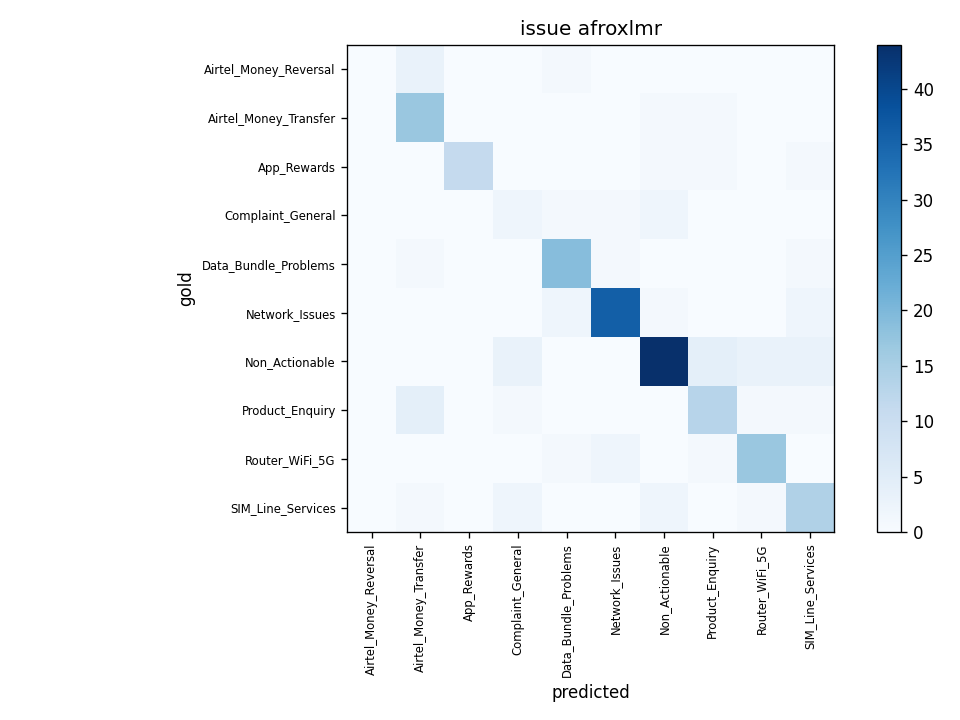
\includegraphics[width=0.78\textwidth]{issue_afroxlmr.png}
\caption{Issue confusion matrix, AfroXLMR.}
\label{fig:issue-cm}
\end{figure}

Paired macro-F1 minus TF-IDF: majority $-0.596$ [$-0.673$, $-0.501$]; keyword $-0.226$ [$-0.360$, $-0.103$]; AfroXLMR $+0.020$ [$-0.062$, $0.117$].

\subsection{Sentiment (\texorpdfstring{$n = 150$}{n = 150})}

Gold support: negative 93, not\_negative 57.

\begin{table}[H]
\centering
\caption{Sentiment-head test macro-F1 with 95\% percentile bootstrap intervals ($n = 150$).}
\begin{tabular}{lrc}
\toprule
model & macro-F1 & 95\% CI \\
\midrule
majority & 0.383 & [0.353, 0.409] \\
keyword  & 0.383 & [0.353, 0.409] \\
tfidf    & 0.758 & [0.685, 0.825] \\
afroxlmr & 0.800 & [0.727, 0.863] \\
\bottomrule
\end{tabular}
\end{table}

TF-IDF per-class F1: negative 0.80 (93), not\_negative 0.71 (57). AfroXLMR: negative 0.84 (93), not\_negative 0.76 (57). Majority and the keyword rule both score 0.77 on negative and 0.00 on not\_negative, which is why their macro-F1 matches.

\begin{figure}[H]
\centering
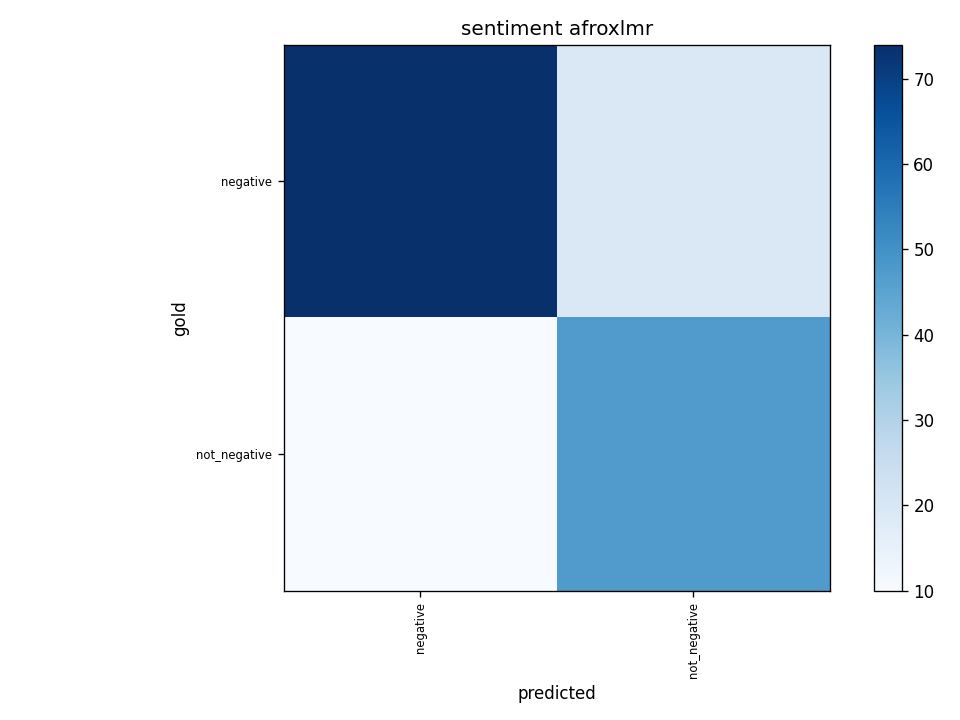
\includegraphics[width=0.72\textwidth]{sentiment_afroxlmr.png}
\caption{Sentiment confusion matrix, AfroXLMR.}
\label{fig:sentiment-cm}
\end{figure}

Paired macro-F1 minus TF-IDF: majority $-0.375$ [$-0.454$, $-0.291$]; keyword $-0.375$ [$-0.454$, $-0.291$]; AfroXLMR $+0.043$ [$-0.017$, $0.099$].

\subsection{Urgency (\texorpdfstring{$n = 120$}{n = 120})}

Gold support: low 17, medium 52, emergency 51 (69 non-emergency).

\begin{table}[H]
\centering
\caption{Urgency-head test metrics with 95\% percentile bootstrap intervals on macro-F1 ($n = 120$).}
\small
\setlength{\tabcolsep}{4pt}
\begin{tabular}{lrrrrr}
\toprule
model & macro-F1 & 95\% CI & QWK & emerg.\ recall & false-emerg.\ rate \\
\midrule
majority & 0.199 & [0.170, 0.227] & 0.000 & 0.000 & 0.000 \\
keyword  & 0.215 & [0.155, 0.272] & 0.044 & 0.000 & 0.043 \\
tfidf    & 0.633 & [0.526, 0.723] & 0.554 & 0.667 & 0.174 \\
afroxlmr & 0.687 & [0.589, 0.770] & 0.687 & 0.804 & 0.145 \\
\bottomrule
\end{tabular}
\end{table}

TF-IDF per-class F1: low 0.48 (17), medium 0.67 (52), emergency 0.74 (51). AfroXLMR: low 0.59 (17), medium 0.67 (52), emergency 0.80 (51).

\begin{figure}[H]
\centering
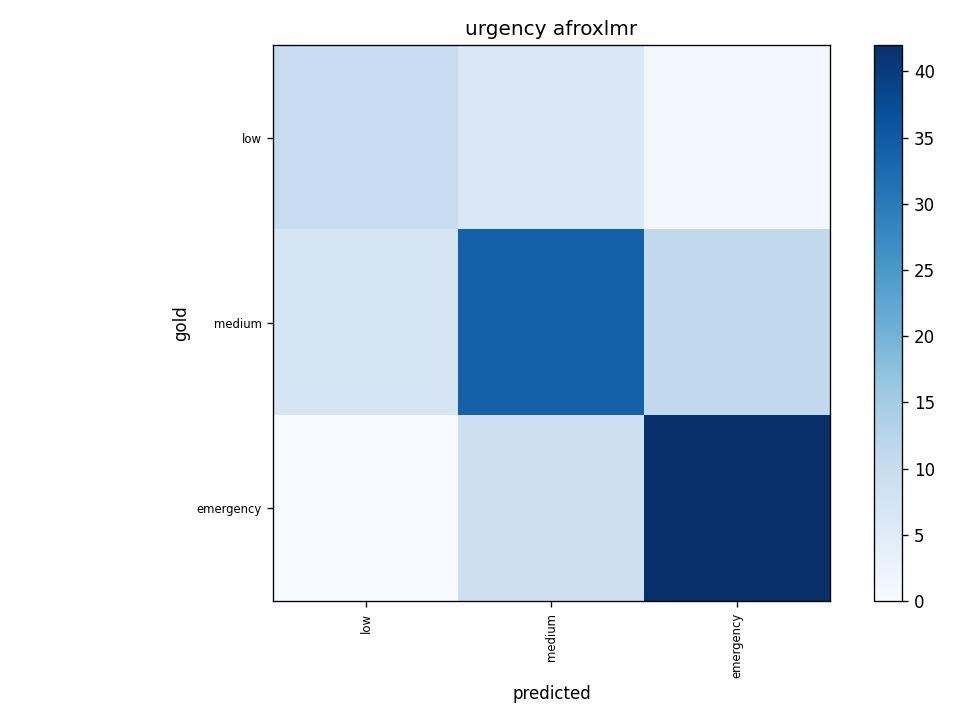
\includegraphics[width=0.72\textwidth]{urgency_afroxlmr.png}
\caption{Urgency confusion matrix, AfroXLMR.}
\label{fig:urgency-cm}
\end{figure}

Paired macro-F1 minus TF-IDF: majority $-0.434$ [$-0.536$, $-0.324$]; keyword $-0.418$ [$-0.511$, $-0.307$]; AfroXLMR $+0.055$ [$-0.020$, $0.135$].

AfroXLMR's point estimate is above TF-IDF on all three heads. The paired bootstrap intervals on those macro-F1 differences all include zero (issue $+0.020$ [$-0.062$, $0.117$], sentiment $+0.043$ [$-0.017$, $0.099$], urgency $+0.055$ [$-0.020$, $0.135$]), so the test sizes do not show a significant macro-F1 gain. Two urgency contrasts do separate: paired QWK $+0.133$ [$0.002$, $0.272$] and paired emergency recall $+0.137$ [$0.036$, $0.259$]. At the validation threshold, test emergency recall is 0.804 against TF-IDF 0.667, and the false-emergency rate is 0.145 against 0.174.

TF-IDF and AfroXLMR are both well above the majority and keyword baselines on every head. The two smallest issue classes, reversal ($n = 4$) and general complaint ($n = 6$), stay weak. Reversal is the class where the transformer loses to TF-IDF.

\section{Limitations}

\begin{itemize}
  \item One seed (42). There is no seed interval around the transformer.
  \item The urgency test is 120 messages. Emergency recall on 51 gold emergencies moves quickly when a few rows flip.
  \item Two issue classes have support 4 and 6. A single error changes their F1 a lot. The bootstrap intervals on issue macro-F1 are wide for that reason.
  \item 688 urgency training rows are silver labels from Groq, not Chris's gold. They are weighted down, but they are still in the training loss.
  \item The encoder is AfroXLMR-base, not large. The frozen fraction matches the proposal; the capacity does not.
  \item The T4 point estimates favour AfroXLMR, and the macro-F1 intervals still include zero. A second seed or a larger test would be needed before calling the gain significant.
\end{itemize}

\section{Real-world relevance}

The queue still has to route a code-switched message, judge the tone, and decide whether it is an emergency. A TF-IDF service already runs without a GPU (\texttt{MODEL\_\allowbreak{}BACKEND=tfidf}). The transformer path is the same API with the checkpoint swapped. Masking is the same function at training and at request time, so the text the model sees does not grow a second copy of a phone number or an ID. Duplicate groups keep a near-copy of a gold emergency out of training.

Clearance status: it is cleared for coursework. The raw export is not in the git repository.

\section{Rubric to artefact}

The capstone is 60\% of the course. Weights are the brief's.

\begin{table}[H]
\centering
\caption{Rubric rows mapped to artefacts in the public repository.}
\begin{tabular}{ll>{\raggedright\arraybackslash}p{8.0cm}}
\toprule
Rubric row & Weight & Where it is \\
\midrule
Data pipeline & 10\% & \texttt{src/\allowbreak{}capstone/\allowbreak{}prepare\_\allowbreak{}data.py}, \texttt{pii.py}, \texttt{duplicates.py}, \texttt{docs/\allowbreak{}label\_\allowbreak{}rubric.md}, real audit counts above \\
Modelling and evaluation & 20\% & \texttt{src/\allowbreak{}capstone/\allowbreak{}models/\allowbreak{}}, \texttt{evaluate.py}, this results section, \texttt{reports/\allowbreak{}results.json} on a real run \\
Technique justification & 10\% & \texttt{docs/\allowbreak{}technique\_\allowbreak{}justification.md} \\
Deployment (API and Docker) & 10\% & \texttt{src/\allowbreak{}capstone/\allowbreak{}serving/\allowbreak{}}, \texttt{Dockerfile}, \texttt{docker-compose.yml}, \texttt{make serve-smoke} \\
Final report and presentation & 10\% & this file \\
Total & 60\% & \\
\bottomrule
\end{tabular}
\end{table}

\end{document}
